\chapter{Lực Lo-ren-xơ}
\section{Lý thuyết trọng tâm}
\subsection{Định nghĩa}
Mọi điện tích chuyển động trong một từ trường, đều chịu tác dụng của lực từ. Lực này gọi là lực Lo-ren-xơ.
\subsection{Xác định lực Lo-ren-xơ}
Lực Lo-ren-xơ do từ trường có cảm ứng từ $\vec{B}$ tác dụng lên một điện tích $q_0$ chuyển động với vận tốc $\vec{v}$ có các đặc điểm:
\begin{itemize}
	\item phương vuông góc với $\vec{v}$ và $\vec{B}$. 
	\item chiều tuân theo quy tắc bàn tay trái: Để bàn tay trái mở rộng sao cho từ trường hướng vào lòng bàn tay, chiều từ cổ tay đến ngón giữa là chiều của $\vec{v}$ khi $q_0>0$ và ngược chiều $\vec{v}$  khi $q_0>0$. Lúc đó, chiều của lực Lo-ren-xơ là chiều ngón cái choãi ra.
	\item độ lớn:
\begin{equation}
f=\left|q_0 \right|vB\sin \alpha.
\end{equation}
\end{itemize}
\begin{center}
	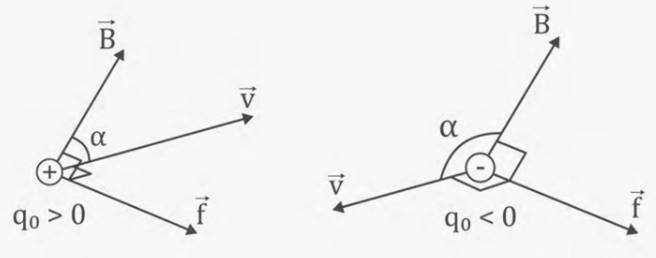
\includegraphics[scale=0.8]{../figs/VN11-PH-27-L-019-1-h72.jpg}
\end{center}
 
\section{Bài tập }
\begin{dang}{Tính các đại lượng trong công thức lực Lo-ren-xơ}
\end{dang}
\textbf{Phương pháp giải}

Sử dụng công thức tính độ lớn lực Lo-ren-xơ:
\begin{equation}
f=\left|q_0 \right|vB\sin \alpha,
\end{equation}

Từ đó suy ra các giá trị độ lớn của $f$, điện tích $q$, cảm ứng từ $B$, vận tốc $v$ và góc $\alpha$ hợp bởi $\vec{v}$ và $\vec{B}$.

\vspace{1em}
\viduii{2}{
Một hạt mang điện tích $q_0=\text{6,4}\cdot 10^{-6}\ \text{C}$ bay vào trong từ trường đều có $B=\text{5}\cdot 10^{-2}\ \text{T}$  hợp với hướng của đường sức từ $30^\circ$. Lực Lo-ren-xơ tác dụng lên hạt có độ lớn $f=\text{3,2}\cdot 10^{-13}\ \text{N}$. Vận tốc của hạt đó khi bắt đầu vào trong từ trường là

\begin{mcq}(4)
	\item $\text{2}\cdot 10^{6}\ \text{m/s}$.
	\item $\text{3}\cdot 10^{6}\ \text{m/s}$.
	\item $\text{4}\cdot 10^{6}\ \text{m/s}$.
	\item $\text{5}\cdot 10^{6}\ \text{m/s}$.
\end{mcq}}{
\begin{center}
	\textbf{Hướng dẫn giải:}
\end{center}

$f=\left|q_0 \right|vB\sin \alpha$.

$\Rightarrow v=\dfrac{f}{\left|q_0 \right|B\sin \alpha}=\text{2}\cdot 10^{6}\ \text{m/s}$.

\textbf{	Đáp án: A.}
}

\viduii{2}{
Một hạt điện tích chuyển động trong từ trường đều quĩ đạo của hạt vuông góc với đường sức từ. Nếu hạt chuyển động với vận tốc $v_1=\text{2,5}\cdot 10^{6}\ \text{m/s}$  thì lực Lo-ren-xơ tác dụng lên hạt có độ lớn là $f_1=\text{2}\cdot 10^{-12}\ \text{N}$, nếu hạt chuyển động với vận tốc là $v_2=\text{3}\cdot 10^{6}\ \text{m/s}$ thì lực Lo-ren-xơ tác dụng lên hạt có giá trị là
\begin{mcq}(4)
	\item $\text{1,1}\cdot 10^{-12}\ \text{N}$.
	\item $\text{2,2}\cdot 10^{-12}\ \text{N}$.
	\item $\text{1,4}\cdot 10^{-12}\ \text{N}$.
	\item $\text{2,4}\cdot 10^{-12}\ \text{N}$.
\end{mcq}}{
\begin{center}
	\textbf{Hướng dẫn giải:}
\end{center}

công thức tính độ lớn lực Lo-ren-xơ: $f=\left|q_0 \right|vB\sin \alpha$.
	
	Lực Lo-ren-xơ tỉ lệ thuận với vận tốc $v$.
	
	$\Rightarrow \dfrac{f_2}{f_1}=\dfrac{v_2}{v_1}=\Rightarrow f_2= f_1\cdot \dfrac{v_2}{v_1}=\text{2,4}\cdot 10^{-12}\ \text{N}$.
	
\textbf{	Đáp án: D.}
	}
\begin{dang}{Xác định phương, chiều lực Lo-ren-xơ}
\end{dang}
\textbf{Phương pháp giải}

Lực Lorenxơ tác dụng lên điện tích $q_0$ đang chuyển động với vận tốc $\vec{v}$trong từ trường có:
\begin{itemize}
	\item Điểm đặt: tại điện tích $q$.
	\item Phương: vuông góc với mặt phẳng chứa $\vec{v}$ và $\vec{B}$. 
	\item Chiều: xác định theo quy tắc bàn tay trái: đặt bàn tay trái mở rộng sao cho từ trường hướng vào lòng bàn tay, chiều từ cổ tay đến ngón giữa là chiều của $\vec{v}$
	\begin{itemize}
		\item Nếu $q>0$: chiều lực Lo-ren-xơ cùng với chiều chỉ của ngón tay cái.
		\item Nếu $q<0$: chiều lực Lo-ren-xơ ngược với chiều chỉ của ngón tay cái.
	\end{itemize}
	
\end{itemize}


\vspace{1em}

\viduii{3}{
Trong các hình vẽ sau, hình vẽ nào chỉ đúng chiều của lực Lo-ren-xơ tác dụng lên các hạt mang điện?

\begin{mcq}(2)
	\item 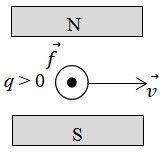
\includegraphics[scale=0.8]{../figs/VN11-PH-27-L-019-1-h74.jpg}
	\item 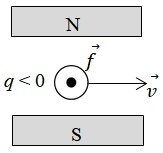
\includegraphics[scale=0.8]{../figs/VN11-PH-27-L-019-1-h75.jpg}
	\item 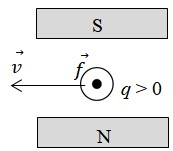
\includegraphics[scale=0.8]{../figs/VN11-PH-27-L-019-1-h76.jpg}
	\item 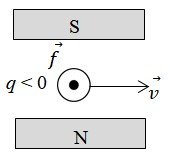
\includegraphics[scale=0.8]{../figs/VN11-PH-27-L-019-1-h77.jpg}
\end{mcq}}{
\begin{center}
	\textbf{Hướng dẫn giải:}
\end{center}

{
Câu A, C, D là sai vì theo quy tắc bàn tay trái thì lực Lo-ren-xơ phải có chiều từ ngoài vào trong mặt phẳng giấy. 

\textbf{Đáp án: B.}
}
}

\viduii{3}{
Trong các hình vẽ sau, hình vẽ nào chỉ đúng chiều vận tốc $\vec{v}$ của hạt mang điện?
\begin{mcq}(2)
	\item 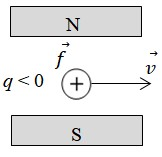
\includegraphics[scale=0.8]{../figs/VN11-PH-27-L-019-1-h78.jpg}
	\item 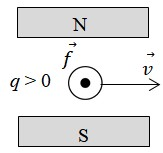
\includegraphics[scale=0.8]{../figs/VN11-PH-27-L-019-1-h79.jpg}
	\item 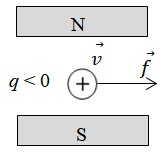
\includegraphics[scale=0.8]{../figs/VN11-PH-27-L-019-1-h80.jpg}
	\item 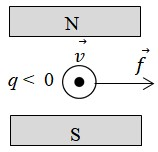
\includegraphics[scale=0.8]{../figs/VN11-PH-27-L-019-1-h81.jpg}
\end{mcq}}
{\begin{center}
	\textbf{Hướng dẫn giải:}
\end{center}

{ Câu A, B là sai vì theo quy tắc bàn tay trái thì vận tốc $\vec{v}$ có chiều từ phải sang trái. 
	
Câu D là sai vì theo quy tắc bàn tay trái thì vận tốc $\vec{v}$ có chiều từ ngoài vào trong mặt phẳng giấy.

\textbf{Đáp án: C.}
}



}
